%%%%%%%%%%%%%%%%%%%%
%                 File Experiment01.tex        %
%                 Experiment M-1               %
%                   Force Table                %
%                                              %
%%%%%%%%%%%%%%%%%%%%

\labChapter{Lab}{Learn to Lab: Domino size \& Density}
\label{lab:M0}

% Introduction
\section*{Introduction}

There are two types of physical quantities: scalars and vectors.  The number of attributes required to define a scalar and a vector distinguishes them.
An example of a scalar quantity is temperature and an example of a vector is a force.
In this laboratory a force table is used to study the vector properties of forces:
\begin{enumerate}
\item[$\triangleright$] how force vectors are added and
\item[$\triangleright$] the concept of forces in equilibrium.
\end{enumerate}













\section{Background}

Differing from a scalar which requires only a single value, positive or negative, a vector is a quantity that is described by a magnitude, direction and units; for example, a force may be $100\,\newton$ in magnitude with direction $90\degree$ counterclockwise from the $x$-axis.   This force is written as $100\,\newton \ @ \ 90\degree$. We will use bold face type to indicate a vector while the regular typeface will indicate the scalar magnitude and the components of the vector.

When several forces act on an object, it is generally desirable to determine the sum of these forces, called the resultant force.  Suppose $\vec{F}_1$ and $\vec{F}_2$ act on a body. The resultant $\vec{R}$ is defined by the vector sum of the two forces, thus
\begin{equation}
   \vec{R} = \vec{F}_1 + \vec{F}_2.
\end{equation}
If many forces act on the body then
\begin{equation}
  \vec{R} = \sum_{i=1}^N \vec{F}_i.
\end{equation}
The resultant force is that single force which can completely replace a number of individual forces acting.  When the resultant force is zero, the object is said to be in equilibrium.

We will consider two methods of vector addition:
\begin{enumerate}
\item[$\triangleright$] The graphical method
\item[$\triangleright$] The method of components
\end{enumerate}

\subsection{Graphical Method}

%Figure01
\begin{figure}%[ht]
  \begin{center}        
    \includegraphics[width=2.6in]{Experiment01Figures/Figure01.pdf}
  \end{center}
  \caption{Two force vectors $\vec{F}_1$ and $\vec{F}_2$}
  \label{M01Fig01}  % the \label command comes AFTER the caption
\end{figure}

Vectors $\vec{F}_1$ and $\vec{F}_2$  (Fig.~\ref{M01Fig01}) are added graphically as follows:
Beginning at a convenient point on a piece of graph paper, usually at the origin of a rectangular coordinate system draw one of the vectors as an arrow to scale and pointing in the proper direction.  Place the second vector with its tail at the tip of the first, again drawn to scale and pointing in the proper direction.  The resultant $\vec{R}$ is the vector drawn from the tail of the first vector to the tip of the second.  The process is illustrated in Fig.~\ref{M01Fig02} demonstrating the addition operation does not depend on the order of addition.  Thus, like scalar addition,
\begin{equation}
  \vec{F}_1 + \vec{F}_2 = \vec{F}_2 + \vec{F}_1 = \vec{R}.
\end{equation}

%Figure02
\begin{figure}%[ht]
  \begin{center}
    \includegraphics[width=2.6in]{Experiment01Figures/Figure02.pdf}
  \end{center}
  \caption{Adding 2 vectors $\vec{F}_1$ and $\vec{F}_2$, using the graphical (``tail-to-tip'') method.}
  \label{M01Fig02}
\end{figure}

It is important that an appropriate scale be selected with which the vectors are drawn (e.g.\ $1\,\newton = 10\,\centi\meter$). The magnitude of $\vec{R}$ is determined using a ruler, and the angle $\theta$ is measured using a protractor.  Since the negative of a vector is merely the vector pointing in the opposite direction, subtraction is addition with the negative vector pointing in the opposite direction.  Errors can be significantly reduced by using a scale that makes the drawing as large as possible. Neatness counts!

% Method of Components
\subsection{Method of Components}

The method of components is a much more useful and quantitatively accurate method of vector addition.  Each vector is resolved into components along the $x-$ and $y$-axes. That is to say, the vector addition of the two components of the vector is the vector itself.  Thus if two vectors are to be added, we add the components along each axis to form the components of the resultant.

%Figure03
\begin{figure}%[ht]
  \begin{center}
    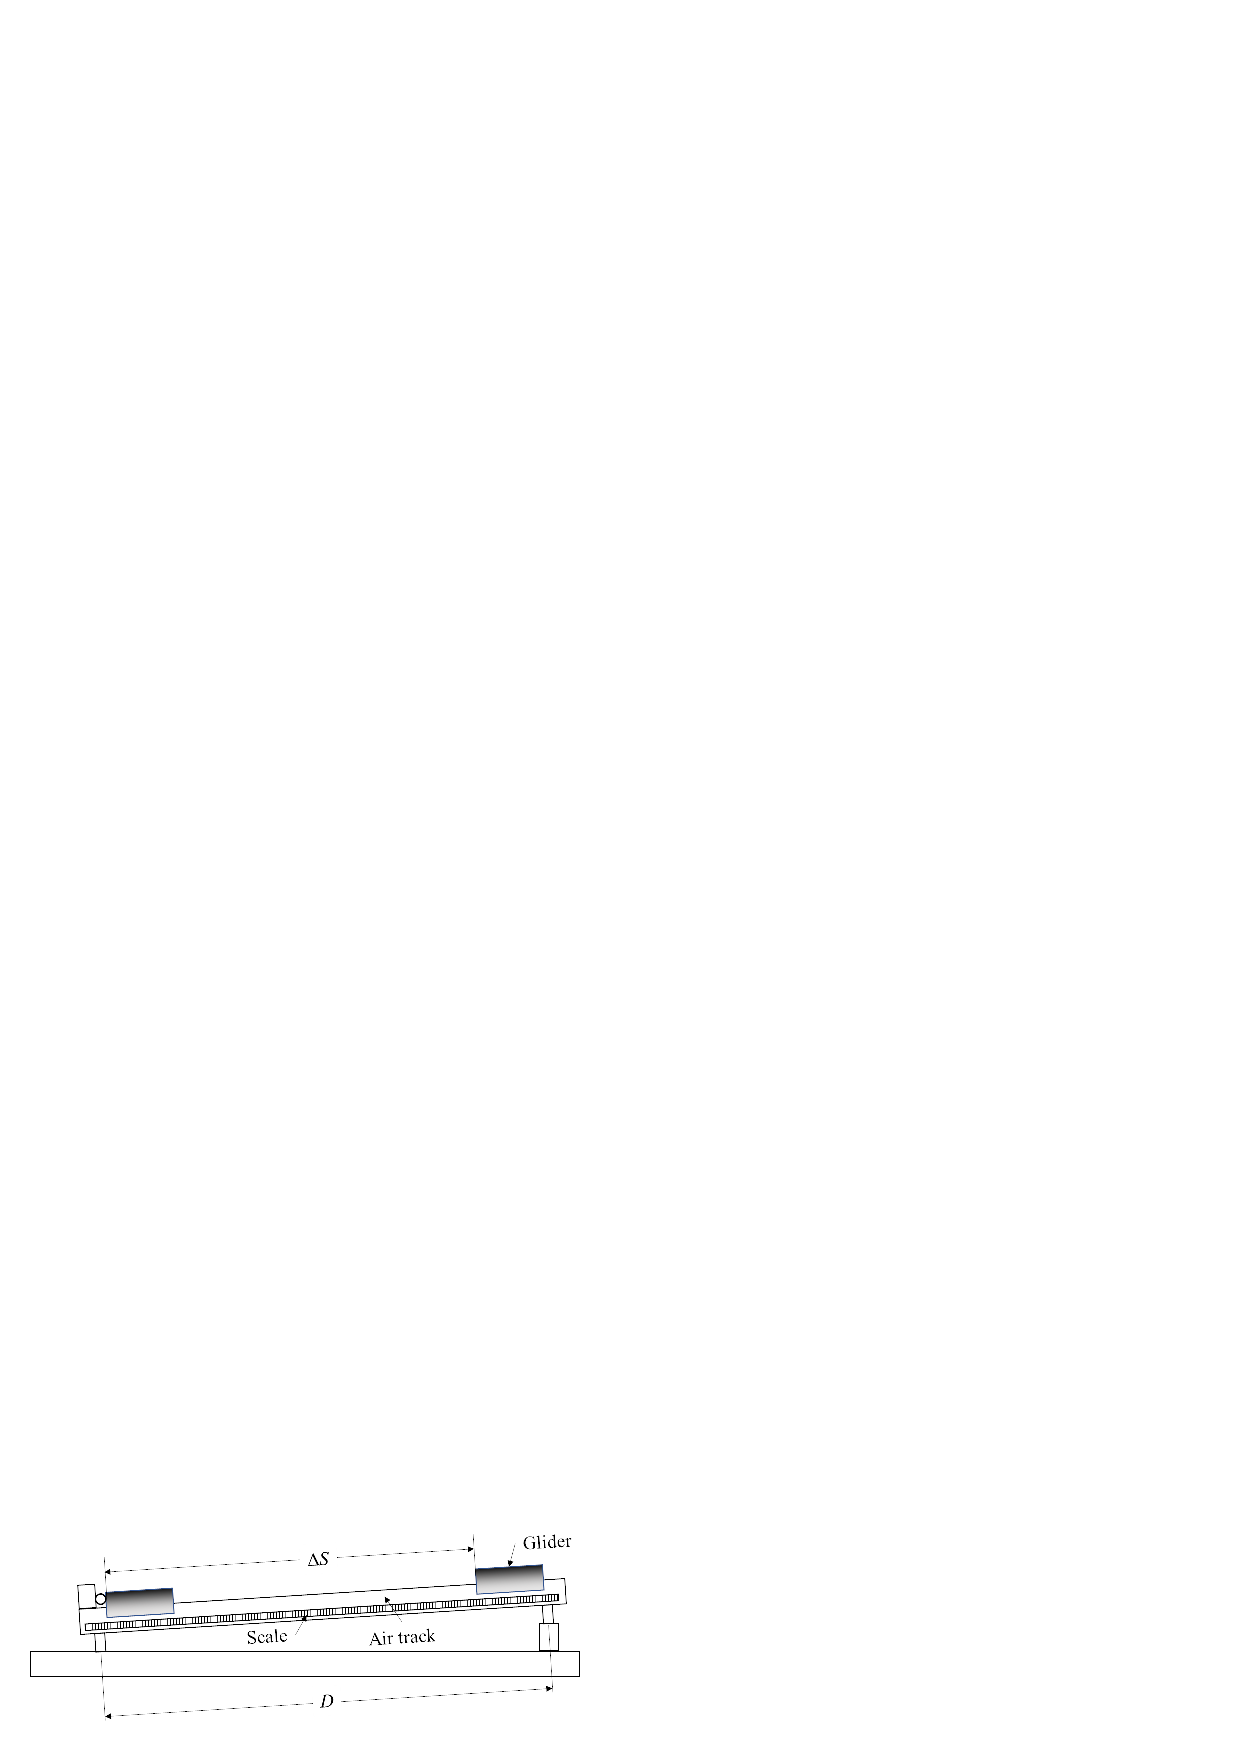
\includegraphics[width=2.6in]{Experiment01Figures/Figure03.pdf}
  \end{center}
  \caption{Adding 2 vectors $\vec{F}_1$ and $\vec{F}_2$ using the method of components. }
  \label{M01Fig03}
\end{figure}

In Fig.~\ref{M01Fig03}, the magnitudes and directions are shown for the two force vectors $\vec{F}_1$ and $\vec{F}_2$ . The magnitudes of the $x$ and $y$ components are calculated for this example as follows:
\begin{equation}
  \begin{aligned} %
    F_{1,x} & = F_1 \, \cos(\theta_{1}) & \qquad F_{2,x} & = F_2 \, \cos(\theta_{2}) \\
            & = 1\,\newton\ \cos(0\degree) = 1\,\newton & &  = 1\,\newton\ \cos(45\degree) = 0.707\,\newton \\
    F_{1,y} & = F_1 \,\sin(\theta_1) & \qquad F_{2,y} & = F_2 \,\sin(\theta_2) \\
            & = 1\,\newton\ \sin(0\degree) = 0\,\newton & &  = 1\,\newton\ \sin(45\degree) = 0.707\,\newton.
  \end{aligned}
\end{equation}
Next, add the $x$-components
\[
  \vec{R}_x = F_{1,x} + F_{2,x} = 1\,\newton + 0.707\,\newton = 1.707\,\newton.
\]
Then, add the $y$-components
\[
  \vec{R}_y = F_{1,y} + F_{2,y} = 0\,\newton + 0.707\,\newton = 0.707\,\newton.
\]
The magnitude of the resultant is found using the relation
\begin{equation}
	\vec{R}^2 = {\vec{R}_x}^2 + {\vec{R}_y}^2,
\end{equation}
or
\[
  \vec{R} = \sqrt{\left(1.707\,\newton\right)^2 +
    \left(0.707\,\newton\right)^2} = 1.848\,\newton.
\]
The angle $\theta$ specifies the direction of the resultant and it can be calculated by noting that
\begin{equation}
  \tan\theta = R_{y} / R_{x}
\end{equation}
and
\begin{align} %
  \theta = \arctan (R_{y} / R_{x}).
\end{align}

For this example illustrated in Fig.~\ref{M01Fig04}
\begin{align} %
  \tan \theta = (0.707\,\newton) / (1.707\,\newton) = 0.414\,\newton,
\end{align}
\begin{align} %
  \theta = \arctan(0.414) = 22.5\degree.
\end{align}

%Figure04
\begin{figure}%[ht]
  \begin{center}
    \includegraphics[width=3.5in]{Experiment01Figures/Figure04.pdf}
  \end{center}
  \caption{Example of $\vec{R}$, the sum of 2 vectors, illustrating $x$- and $y$-components, a well as its magnitude and angle with the $x$-axis.}
  \label{M01Fig04} 
\end{figure}

In this laboratory, an object will be presented with two known forces acting on it.  Equilibrium will be established by adding a third force $\vec{F}_3$, such that the sum of the three forces is zero. Thus we must find the resultant of the two given forces $\vec{F}_1$ and $\vec{F}_2$, and find the force $\vec{F}_3$ that is equal in magnitude and opposite in direction to the resultant of $\vec{F}_1$ and $\vec{F}_2$.  This is illustrated in Fig.~\ref{M01Fig05}.

%Figure05
\begin{figure}%[ht]
  \begin{center}
    \includegraphics[width=4.0in]{Experiment01Figures/Figure05.pdf}
  \end{center}
  \caption{Illustration of the method to determine the force $\vec{F}_{3}$ needed to balance two given forces $\vec{F}_{1}$ and $\vec{F}_{2}$.}
  \label{M01Fig05}
\end{figure}

Here $\vec{F}_3$ is the force necessary to equilibrate $\vec{F}_1$ and $\vec{F}_2$.  Note that, the resultant of $\vec{F}_1+\vec{F}_2+\vec{F}_3$ is zero since the ring is in equilibrium.

Force $\vec{F}_3$ has the same magnitude as the resultant $\vec{R}$, but acts in a direction opposite to $\vec{R}$ (recall that $\vec{R}=\vec{F}_1+\vec{F}_2$).  So we now have
\begin{equation}
  \vec{F}_3 = -\vec{R}.
\end{equation}
We conclude that the force necessary to equilibrate two or more forces is equal and opposite to the resultant of the two (or more) forces.














\section{Experimental Procedure}

The apparatus for this experiment consist of a force table, weight holders, and weights.  The force table consists of a circular metal tabletop mounted on a vertical rod held in a tripod support with leveling screws.  The rim of the circular top has a $360\degree$ scale engraved on it along which it is possible to clamp a number of pulleys.  At the center of the table is a small ring held in place by means of a removable pin.  The ends of three cords are tied to the ring with each cord leading over a pulley and ending with a weight holder tied to its other end.  When the forces along the cords acting upon the small ring are balanced, or in static equilibrium, the ring remains stationary.  For accurate measurements of the angles involved, each cord must be aimed directly at the center of the ring requiring that the equilibrium condition must be established when the ring is exactly centered on the table.

In the laboratory three different cases will be assigned. A fourth case involves determining unknown masses by balancing the force from a known mass. For each of the first three cases, two masses, each at a specific angle will be specified.  Each mass, consisting of a $50\,\gram$ hanger plus the necessary additional mass, will be hung from a cord routed over a pulley at the assigned angular positions and finally tied to the ring.  A third cord, hanger, and pulley assembly is put in place for the third, unknown force.  Each force is the weight of the hanging mass at the pulley angle.  Determine the unknown forces for each of the three cases.  After you determine the unknown force in the third case, tilt the force table and determine any change in the third force with the tilted table.

If, for example, you are given the following case to work with
\[
\begin{array}{rll}
  \mbox{Mass \#1:} & 200\,\gram & \mbox{@}\,0\degree \\
  \mbox{Mass \#2:} & 250\,\gram & \mbox{@}\,135\degree.
\end{array}
\]
Place a pulley at $0\degree$ and add $150\,\gram$ to the $50\,\gram$ weight hanger.  The tension on the cord is the same on both sides of the pulley so that the downward pull of gravity on the hanger and masses is equal to the tension in the cord leading to the ring.  Thus,
\[
\vec{F}_1 = m g = 0.20\,\kilo\gram\times 9.8\,\meter\per\second\squared
         = 1.96\,\newton\ @\ 0\degree.
\]
Similarly, add $200\,\gram$ to a $50\,\gram$ weight hanger and run its cord over a pulley mounted at $135\degree$.
\[
\vec{F}_2 = m g = 0.25\,\kilo\gram\times 9.8\,\metre\per\second\squared
         = 2.45\,\newton\ @ \ 135\degree.
\]

Having established the given magnitudes and directions for each of the given forces, $\vec{F}_{1}$ and $\vec{F}_{2}$, adjust both the amount of mass hanging on cord 3 and its angular position so that the ring is stationary at the center of the table.  In order for angular measurements to be accurate, each cord must be on a line through the center of the table.  Sighting along each cord towards the center pin easily and accurately checks this on the table.

Record the angular position and total mass required to balance $\vec{F}_{1}$ and $\vec{F}_{2}$.  The magnitude of the balancing force $\vec{F}_{3}$ is the total weight hanging.

\subsection{Finding Unknown Masses}

In this case you will experimentally determine two unknown masses by balancing the $x$ and $y$ components of the force of a known mass.
Place the pulley with the known mass $M_1 = 50\,\gram $ at $\theta_1 = 0\degree$.
Determine the angles $\theta_2$ and $\theta_3$ for unknown masses $M_2$ and $M_3$ that result in the ring being in equilibrium.

First find $M_2$ and $M_3$ using the graphical method.
Accurately draw $ \vec{F}_1$ on graph paper using an appropriate scale.
Draw a line in the direction of $\vec{F}_2$ at angle $\theta_2$ through the head of $\vec{F}_1$.
Draw a line in the direction of $\vec{F}_3$ at angle $\theta_3$ through the tail of $\vec{F}_1$.
Find the point where these two lines intersect to form a triangle representing equilibrium of the three forces.
Determine the magnitude of $\vec{F}_2$ and $\vec{F}_3$ using your selected scale by measuring the sides of the triangle.
Find the unknown masses by dividing by $g$.

Now calculate the unknown masses using the method of components.
You have to solve a pair of equations for the $x$ and $y$ components of force.
This calculation is the algebraic version of finding the intersection of the two lines in the graphical method.
The equation for equilibrium in the $x$ direction is
\begin{equation}
  \label{eq:M01unknownx}
  (M_1 + M_2 \cos\theta_2 + M_3 \cos\theta_3)g = 0.
\end{equation}
The equation for equilibrium in the $y$ direction is
\begin{equation}
  \label{eq:M01unknowny}
  (M_2 \sin\theta_2 + M_3 \sin\theta_3)g = 0.
\end{equation}
$M_2$ is eliminated by multiplying the $x$ component by $\sin \theta_2$ and subtracting the $y$ component multiplied by $\cos \theta_2$
\begin{equation}
  \label{eq:M01solveM3}
  M_1 \sin \theta_2  + M_3 \cos \theta_3 \sin \theta_2 - M_3 \sin \theta_3 \cos \theta_2 = 0.
\end{equation}
Using the known values, solve for $M_3$ and enter the value in the table.

Similarly, eliminating $M_3$ gives
\begin{equation}
  \label{eq:M01solveM2}
  M_1 \sin \theta_3  + M_2 \cos \theta_2 \sin \theta_3 - M_2 \sin \theta_2 \cos \theta_3 = 0.
\end{equation}
Using the known values, solve for $M_2$ and enter the value in the table.

Measure $M_2$ and $M_3$ on the scale and enter the values in the table.














\section{Data Analysis}

Data analysis includes estimated or calculated errors. See the guidance starting at page \ref{sec:TypesErrors}.

\begin{itemize}
\item[$\triangleright$] Create a table with common data such as the accepted value of $g$, the mass of the holder and any other common data you need for the cases. You will reference this table in the calculations.
\item[$\triangleright$] The data layout for each of the first three cases is the same. Create a table with a row for each of the three applied forces with:
    \begin{itemize}
      \item the mass in kilograms,
      \item the calculated magnitude of the force in Newtons,
      \item the direction of the force in degrees,
      \item the calculated $x$-component of the force in Newtons,
      \item the calculated $y$-component of the force in Newtons,
      \item your estimate of the magnitude of the experimental error of the forces in Newtons, and
      \item your estimate of the experimental error of the angle.
    \end{itemize}
\item[$\triangleright$] Create a table to analyze the results of your measurements. The columns could include
    \begin{itemize}
      \item the $x$ and $y$ components of the resultant of the two given forces $\vec{F}_1$ and $\vec{F}_2$,
      \item the direction and magnitude of the resultant $\vec{R} = \vec{F}_1 + \vec{F}_2$,
      \item the vector components of the measured total force, which is the vector sum of $\vec{R}$ and $\vec{F}_3$, and
      \item the magnitude of the total force. The total force should be zero because the ring is in equilibrium. The magnitude of the total force therefore is a measure of the experimental error.
    \end{itemize}
\item[$\triangleright$] The fourth case with unknown masses requires a table with some differences. In this case you will calculate the unknown masses using the fact that the components of the force balance. Create a table including:
    \begin{itemize}
      \item The known mass $M_1$,
      \item the $x$ and $y$ components of the force from $M_1$,
      \item the experimental angle of the forces from $M_2$ and $M_3$,
      \item the experimental values of $M_2$ and $M_3$ from Eqn.~\ref{eq:M01solveM3} and Eqn.~\ref{eq:M01solveM2},
      \item the experimental values of $M_2$ and $M_3$ from graphical analysis, and
      \item the values of $M_2$ and $M_3$ as measured on a triple-beam balance.
    \end{itemize}
\end{itemize}

It is good practice to complete the analysis of the first case before beginning the next case. If you have some error in your experimental method or in your calculation, you can correct it before completing all the other cases. The layout of the rows for the further cases can then be created by copying the first case.














% Experimental Procedure
\section{Interpretation of Results}

\begin{itemize}
\item[$\triangleright$] Find the resultant force for each of the three experimental cases. Using the method of components, find the magnitude and direction of this resultant $\vec{R}$.  The balancing force $\vec{F}_{3}$ equals the negative of resultant $\vec{R}$ of $ \vec{F}_{1}$ and $\vec{F}_{2}$, i.e.\ the direction of $\vec{F}_{3}$ is $180\degree$ from $\vec{R}$.
\item[$\triangleright$] For one of the cases, plot the vectors $\vec{F}_{1}$ and $\vec{F}_{2}$.  Graphically construct and draw the vector $\vec{R}$.  From $\vec{R}$, construct the expected $\vec{F}_{3}$.  On the same graph, plot your experimentally determined vector $\vec{F}_{3}$ and compare the two $\vec{F}_{3}$ vectors.
%          Calculate the \% difference in the magnitudes of the two vectors using the following relation:
%	\begin{align} %
%	\mbox{\% Difference} = \frac{\mbox{Experimental} \ \mbox{Value} - \mbox{Calculated} \ \mbox{Value}}{\mbox{Calculated} \ \mbox{Value}} \times 100\%.
%	\end{align}
\item[$\triangleright$] Discuss in your lab report any discrepancy in the directions of the two vectors as well as their magnitude.
\item[$\triangleright$] Assume the force table is not level while you perform the experiment. Discuss the effect this would have on the outcome of your measurement of the equilibrium force $\vec{F}_{3}$. To determine this, tilt the balanced force table for one of the cases. Discuss the outcome among yourselves and with your lab instructor.
\end{itemize}

